\documentclass[a4paper]{article}
\usepackage[utf8]{inputenc}
\usepackage[spanish, es-tabla, es-noshorthands]{babel}
\usepackage[table,xcdraw]{xcolor}
\usepackage[a4paper, footnotesep = 1cm, width=20cm, top=2.5cm, height=25cm, textwidth=18cm, textheight=25cm]{geometry}
%\geometry{showframe}

\usepackage{tikz}
\usepackage{amsmath}
\usepackage{amsfonts}
\usepackage{amssymb}
\usepackage{float}
\usepackage{graphicx}
\usepackage{caption}
\usepackage{subcaption}
\usepackage{multicol}
\usepackage{multirow}
\setlength{\doublerulesep}{\arrayrulewidth}
\usepackage{booktabs}
\usepackage{mathrsfs,amsmath}
\usepackage{hyperref}
\hypersetup{
    colorlinks=true,
    linkcolor=blue,
    filecolor=magenta,      
    urlcolor=blue,
    citecolor=blue,    
}

\newcommand{\quotes}[1]{``#1''}
\usepackage{array}
\newcolumntype{C}[1]{>{\centering\let\newline\\\arraybackslash\hspace{0pt}}m{#1}}
\usepackage[american]{circuitikz}
\usetikzlibrary{calc}
\usepackage{fancyhdr}
\usepackage{units} 

\graphicspath{./Imagenes}

\pagestyle{fancy}
\fancyhf{}
\lhead{22.05 ASSD}
\rhead{Mechoulam, Lambertucci, Rodriguez, Londero}
\rfoot{Página \thepage}

\begin{document}

La síntesis aditiva consiste en formar el sonido de un instrumento sumando todas las señales sinusoidales por las cual este está formado. Si bien existen muchas nomenclaturas que refieren a lo mismo, a lo largo de esta implementación se utilizarán las denominaciones \textit{primer armónico} como la componente de menor frecuencia de un sonido; \textit{segundo, tercero, ..., n armónico} como las componentes de frecuencia múltiplos del primer armónico del sonido; y \textit{sobretonos} como cualquier componente de frecuencia del sonido mayor al primer armónico que no es múltiplo de este.

\subsection{Grupos armónicos}

Se sintetizó en una primera instancia al órgano. El órgano es un instrumento muy versátil con un amplio rango de sonidos diferentes, dado que estos están frecuentemente formados por miles de tubos metálicos, abiertos o cerrados. Estos tubos suelen estar agrupados en rangos de manera tal que estos simulen otros instrumentos de viento, como la flauta, el clarinete, el bassoon, el cor anglais, y muchos más. Se puede observar que el órgano es un sintetizador aditivo natural, dado que cada uno de los tubos posee un único tono y timbre, junto a sus armónicos. Es por esta razón que se decidió sintetizar a este instrumento. 

Sin embargo, un órgano de hoy en día posee alrededor de 20000 tubos y 300 rangos distintos. Como sería muy difícil sintetizar a cada tubo por separado, se decidió sintetizar al instrumento de una manera versátil, emulando al instrumento. Se agruparon a los armónicos y sobretonos del instrumento dada una sola nota de frecuencia $f_0$ en los siguientes grupos:

\begin{table}[H]
\centering
\begin{tabular}{@{}ll@{}}
\toprule
\textbf{Grupo armónico} & Frecuencias \\ \midrule
Fundamental & $\sum_{i = 1}^{\infty} f_0 + 2\cdot i \cdot f_0$ \\ 
Quinta & $\sum_{i = 1}^{+\infty} 3f_0 + 6\cdot i \cdot f_0$ \\ 
 Primaria& $\sum_{i = 1}^{+\infty} 2f_0 + 4\cdot i \cdot f_0$ \\ 
 Octava& $\sum_{i = 1}^{+\infty} 4f_0 + 8\cdot i \cdot f_0$ \\ 
 Duodécima& $\sum_{i = 1}^{+\infty} 6f_0 + 12\cdot i \cdot f_0$ \\ 
 Decimoquinta& $\sum_{i = 1}^{+\infty} 8f_0 + 15\cdot i \cdot f_0$ \\ 
 Decimoséptima& $\sum_{i = 1}^{+\infty} 9f_0 + 17\cdot i \cdot f_0$ \\ 
 Decimonovena& $\sum_{i = 1}^{+\infty} 20f_0 + 19\cdot i \cdot f_0$ \\ 
 Tercera mayor& $\sum_{i = 1}^{+\infty} f_0 \cdot 2^{\frac{4}{12}} + 2\cdot i \cdot f_0$ \\ 
 Cuarta perfecta& $\sum_{i = 1}^{+\infty} f_0 \cdot 2^{\frac{5}{12}} + 2\cdot i \cdot f_0$ \\ 
 Quinta perfecta& $\sum_{i = 1}^{+\infty} f_0 \cdot 2^{\frac{7}{12}} + 2\cdot i \cdot f_0$ \\ \bottomrule
\end{tabular}
\end{table}

Asimismo, se permite configurar la cantidad de armónicos que se añaden del grupo fundamental, y la cantidad de armónicos que se añaden del resto. A partir de estos parámetros, se sintetizaron dos configuraciones distintas, las de flauta, y las de órgano entero, mostrado a continuación:

\begin{multicols}{2}
\begin{table}[H]
\centering
\begin{tabular}{@{}ll@{}}
\toprule
\textbf{Grupo armónico} & \textbf{Proporción} \\ \midrule
Fundamental & $0.3$ \\ 
Quinta & $0$ \\ 
 Primaria& $0.65$ \\ 
 Octava& $0$ \\ 
 Duodécima& $0$ \\ 
 Decimoquinta& $0$ \\ 
 Decimoséptima& $0$ \\ 
 Decimonovena& $0$ \\ 
 Tercera mayor& $0.03$ \\ 
 Cuarta perfecta& $0$ \\ 
 Quinta perfecta& $0.02$ \\ \bottomrule
\end{tabular}
\end{table}
\begin{table}[H]
\centering
\begin{tabular}{@{}ll@{}}
\toprule
\textbf{Grupo armónico} & \textbf{Proporción} \\ \midrule
Fundamental & $0.15$ \\ 
Quinta & $0.11$ \\ 
 Primaria& $0.17$ \\ 
 Octava& $0.13$ \\ 
 Duodécima& $0.11$ \\ 
 Decimoquinta& $0.095$ \\ 
 Decimoséptima& $0.095$ \\ 
 Decimonovena& $0.13$ \\ 
 Tercera mayor& $0.005$ \\ 
 Cuarta perfecta& $0.003$ \\ 
 Quinta perfecta& $0.002$ \\ \bottomrule
\end{tabular}
\end{table}
\end{multicols}

\subsection{Ruido}

De vital importancia en la sintetización de instrumentos a la hora de lograr un mayor realismo, y más aun así en instrumentos de viento es el ruido. Se utilizó para esto ruido binario, el cual es superpuesto a cada nota generada por el sintetizador, logrando así un mayor realismo.

\subsection{Ventana temporal}

Se basó la ventana temporal utilizada en esta implementación en la clásica ventana ADSR. Sin embargo, al sintetizarse un instrumento de viento, se fijó el parametro de delay como nulo y el de sustain como unitario. Luego, en vez de realizar la ventana a trozos linealmente, se utilizaron subidas y bajadas exponenciales con una oscilación en el periodo de sustain, el cual se utiliza para simular la técnica de \textit{vibratto} en los instrumentos de vientos generada por tanto vibraciones de la fuente de aire como en la embocadura del instrumento, como se observa en la Figura (\ref{vib}). La frecuencia o incluso existencia de estas vibraciones dependen de la longitud de la nota $T$. Luego, los parámetros que se le pide al usuario son los de $A$ para \textit{Attack}, $R$ para \textit{Release} y $H$ para \textit{Oscillation}, quedando finalmente definida la ventana mediante la fórmula a trozos:

\begin{equation}
   \left\{
\begin{array}{ll}
      -e^{-t \cdot \left( \frac{10F}{A\cdot T} \right) } + 1 & 0\leq t \leq \frac{A \cdot T}{F} \\
      \\
     \left( 1 + \left( \frac{2}{1 + e ^{-\cdot T \cdot \left( t - \frac{A \cdot T}{F} \right) }} - 1 \right) \cdot H \cdot sin\left( 2\pi \cdot \left( t - \frac{A \cdot T}{F} \right) \frac{4T}{\frac{T}{F} \cdot \left( 1 - R - A \right)} \right) \right) & \frac{A \cdot T}{F} \leq x \leq T\cdot (1-\frac{R}{F}) \\
      \\
      -e^{t \cdot \left( \frac{10F}{R\cdot T} \right) } + 1 & T\cdot (1-\frac{R}{F}) \leq t \leq T \\
\end{array} 
\right. 
\end{equation}

donde

\begin{equation}
F = \frac{2}{1 + e^{-\frac{f}{10\cdot f_0}}} \cdot \left( V + 0.5 \right)
\end{equation}

Siendo $V$ la velocity de la nota normalizada de $0$ a $1$, $f_0$ la frecuencia fundamental de la nota y $f$ la frecuencia del armónico al cual se le aplica la ventana. Se puede observar que la ventana crece y decrece más rápido proporcional a la razón entre la frecuencia del armónico y la frecuencia fundamental de la nota, mientras que la ventana crece y decrece más rápido inversamente proporcional a la velocity de la nota. Esto quiere decir que los sonidos más graves reaccionarán más lento, mientras que los agudos se percibirán más rápido. Además, si una nota se toca con una velocity baja, habrá un transitorio más largo entre la máxima y mínima amplitud de la nota.

\begin{figure}[H]
	\centering
	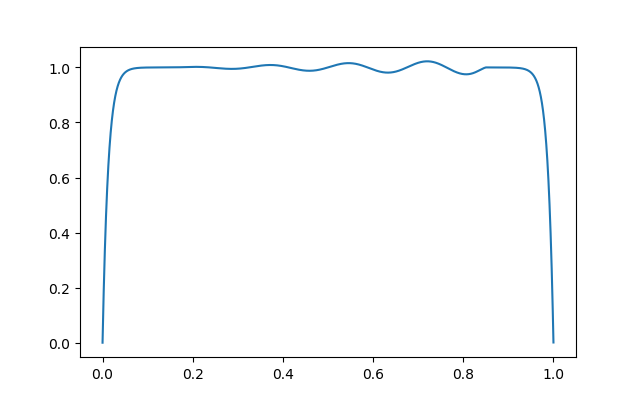
\includegraphics[width=0.7\textwidth]{ImagenesEjercicio2/adsr.png}
	\caption{Ventana temporal para $T = 1$, $A = 0.1$, $R = 0.1$, $H = 0.08$ y $F = 1$.}
	\label{vib}
\end{figure}

Por último, se utilizó una función sigmoidea modificada, la cual mapea valores dentro del intervalo $[0, +\infty)$ al intervalo $[0, 1)$, con el fin de que las oscilaciones en la fase de sustain aparezcan de manera incremental, como suele suceder naturalmente con el vibratto.

\subsection{Caída de armónicos en frecuencia}

Al añadir un grupo de armónicos al instrumento, se puede pensar como que se agrega una nueva frecuencia fundamental junto a sus armónicos, sin embargo, estos armónicos no tienen la misma amplitud que su fundamental, sino que decrecen linealmente en una escala logarítmica. La pendiente de esta envolvente lineal fue hallada observando el espectro de varias notas de instrumentos reales.

Además, esta pendiente decae con la frecuencia, lo que fue experimentalmente hallado como una mejora.

\end{document}